\documentclass{beamer}


\definecolor{grislindo}{rgb}{0.2,0.2,0.2}
\definecolor{claro}{RGB}{255,255,117}
\definecolor{verdeclaro}{RGB}{28,204,130}
\definecolor{verdecito}{RGB}{00,70,60}
\definecolor{verdeoscuro}{RGB}{34,178,117}
\definecolor{lilaclaro}{RGB}{204,61,255}
\definecolor{lilao}{RGB}{50,01,43}
\definecolor{lilita}{RGB}{107,61,104}
\definecolor{crema}{RGB}{255,206,86}
\definecolor{lilaoscuro}{RGB}{138,25,178}
\definecolor{griscl}{rgb}{0.5,0.5,0.5}
\definecolor{grisosc}{RGB}{38,36,36}
\definecolor{griscl2}{RGB}{60,59,59}
\usecolortheme[named=lilita]{structure}
\usetheme{Rochester}

\usepackage[utf8]{inputenc}
%\usepackage{default}
%paquetes-----
%\usepackage{fontspec}
%\usepackage{emerald}
%\usepackage[T1]{fontenc}
%\usepackage[latin1]{inputenc}
\usepackage{float}
\usepackage{mathptmx}
\usepackage{natbib}
\usepackage{graphicx}
\usepackage[spanish]{babel} 
\usepackage{amsmath}
\usepackage{amssymb}
\usepackage{amsfonts}
\usepackage{array}
\usepackage{xcolor}
%\usepackage{wrapfig}
\usepackage{multirow}
%\usepackage{fancybox}
%\usepackage[many]{tcolorbox}
%\usepackage{enumitem}
%\usepackage{xcolor}
%\usepackage{tikz}
%\usepackage{graphicx}
%\usepackage{pst-node}
\usepackage{anyfontsize}
\usepackage[percent]{overpic}
%\usepackage{smartdiagram}
%\usepackage{pbox}
%\usepackage{natbib}
%\usepackage{fontspec}
\usepackage[document]{ragged2e}
%\usepackage[symbol]{footmisc}
%\usetikzlibrary{shapes,arrows}
%\usetikzlibrary{mindmap,trees}
%\usetikzlibrary{calc}
%\usetikzlibrary{backgrounds}
\usefonttheme{structuresmallcapsserif}

\decimalpoint
%\renewcommand{\thefootnote}{\fnsymbol{footnote}}
%\renewcommand*{\thefootnote}{\fnsymbol{footnote}}

\newcounter{daggerfootnote}
\newcommand*{\daggerfootnote}[1]{%
    \setcounter{daggerfootnote}{\value{footnote}}%
    \renewcommand*{\thefootnote}{\fnsymbol{footnote}}%
    \footnote[2]{#1}%
    \setcounter{footnote}{\value{daggerfootnote}}%
    \renewcommand*{\thefootnote}{\arabic{footnote}}%
    }


\title[Título corto]{DISCOS DE ACRECIÓN}
\subtitle{} % Opcional
\author{FERRARO, MARÍA EUGENIA}
\institute{} % Opcional

\begin{document}
\begin{frame}
\titlepage
\end{frame}
%Trasparencias


\begin{frame}
\frametitle{qué entendemos por acreción}
\begin{columns}
\begin{column}{0.60\textwidth}
 \justify
 \vspace{-0.7cm}
 Es el proceso en el que la materia se acumula debido a la gravedad, formando una estructura
 parecida a un disco, también puede formar objetos masivos. Es  
 responsable de la aparición de la mayoría de los objetos en el universo. Casi todos los 
 objetos astronómicos, desde planetas y estrellas hasta galaxias enteras se formaron a 
 través de este proceso. También alimenta algunos de los fenómenos más energéticos 
 observados en el universo. En general, la materia de acreción forma un disco alrededor 
 del objeto central debido a la conservación del momento angular del a materia 
\end{column}
\begin{column}{0.4\textwidth}
 {\it \textcolor{lilita}{ACRECIÓN EN EL UNIVERSO:}}
 Cygnus X-1, un sistema binario de rayos X extensamente estudiado, SS 433, otro binario
 conocido por su disco y precesión de jets, Sagittarius A *, el agujero negro supermasivo 
 en el centro de nuestra galaxia, y M104 , una galaxia espiral que posee un agujero negro 
 inusualmente grande en su centro
\end{column}
\end{columns}
\end{frame}



\begin{frame}
\frametitle{discos de acreción}
\begin{columns}
\begin{column}{1\textwidth}
 \justify
Las partículas atrapadas por la atracción gravitacional de un objeto masivo raramente
viajan directo hacia el objeto central. Por lo general, cada partícula tiene un momento
angular que debe perder para caer hacia el interior. Observando el momento angular
para una órbita circular:
\begin{equation*}
 \vec{L}=\vec{r}\times m\vec{v}
\end{equation*}
vemos que para que r disminuya, ergo, se acerque la partícula hacia el centro,
L debe disminuir (suponiendo la masa constante). \textcolor{lilaoscuro}{\textit
{Como el momento debe conservarse,
solo se puede transferir a otro lugar. Resulta que durante la acreción el momento angular
\textbf{\textit{ se transfiere por fricción}} y se mueve hacia afuera ya que la mayor parte de la
materia que compone al disco se mueve hacia adentro.}}
\end{column}
\begin{column}{0.0\textwidth}
\end{column}
\end{columns}
\end{frame}




\begin{frame}
\frametitle{discos de acreción}
\begin{columns}
\begin{column}{0.5\textwidth}
\hspace*{-1cm} 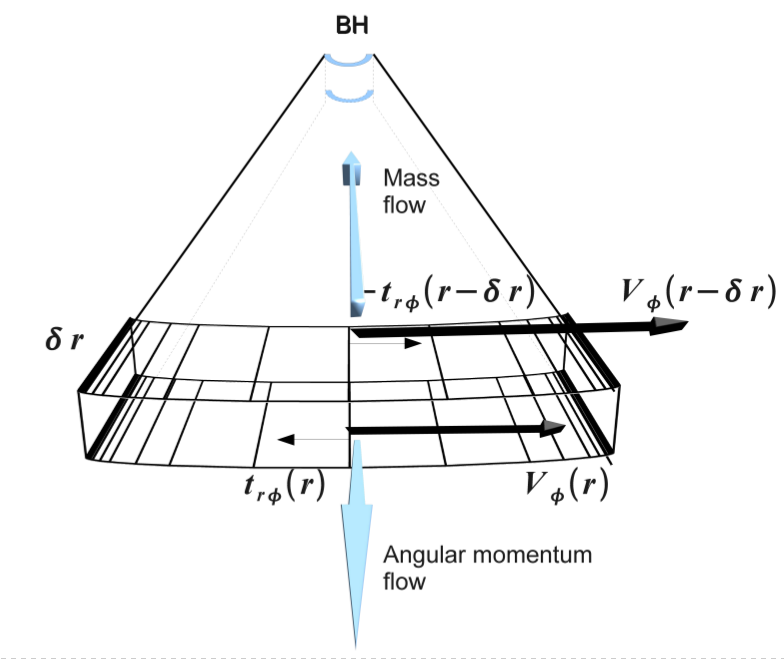
\includegraphics[width=6.5cm,height=5cm]{modelo.png}
\end{column}
\begin{column}{0.5\textwidth}
\justify
\scriptsize
La idea central de los discos de acreción radica en el hecho de que 
las masas de acreción poseen una cantidad considerable de momento
angular por unidad de masa, el cual debe ser eliminado para que las
mismas puedan acumularse en el objeto central. \textit{\textcolor{lilaoscuro} {La pérdida de momento
angular es causada por la \textbf{fricción debida a la viscosidad turbulenta}
que trabaja entre capas de gas adyacentes en el disco}}. La capa interna 
más rápida pierde impulso angular y cae ligeramente, mientras que la
siguiente capa externa (más lenta) gana momento angular, que se entrega
a la siguiente capa externa, y así sucesivamente, lo que resulta en un
flujo continuo hacia el centro mientras se transporta impulso angular
a la región exterior.\\
La fricción del disco calienta al gas, dando
como resultado una emisión continua de radiación.
\end{column}
\end{columns}
\end{frame}



\begin{frame}
\frametitle{discos de acreción en sistemas binarios}
\begin{columns}
\begin{column}{0.6\textwidth}
\hspace*{-0.4cm}
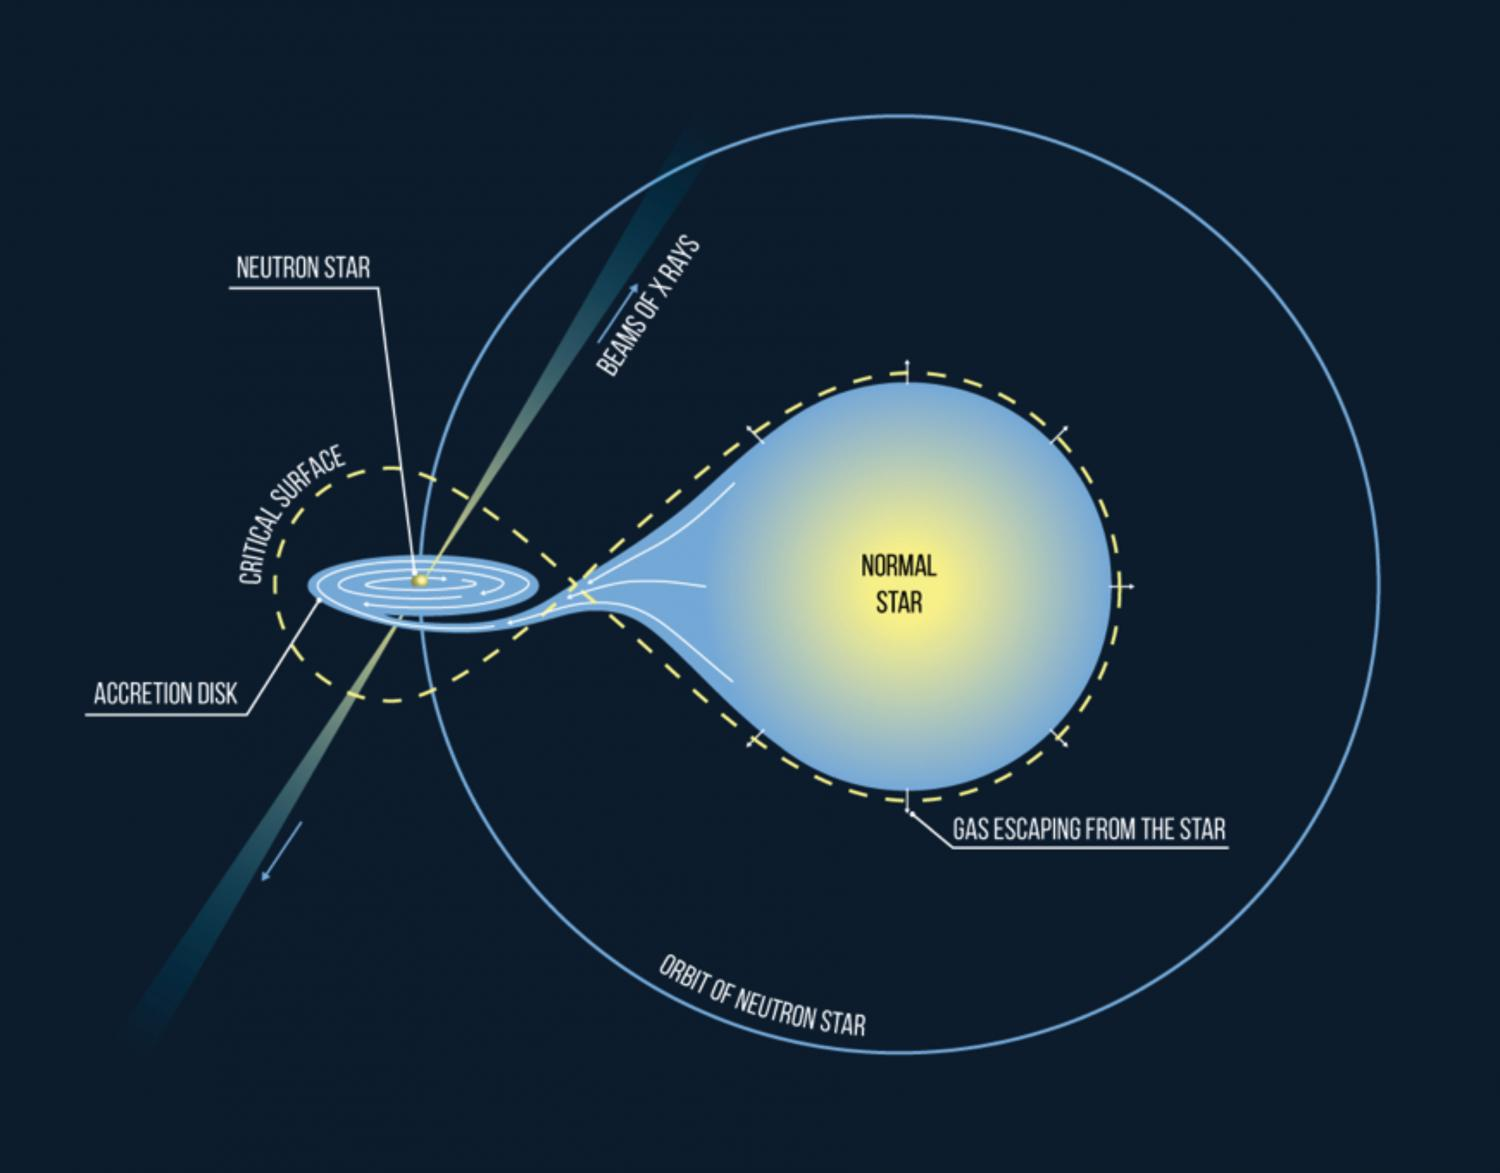
\includegraphics[width=9.0cm, height=7.3cm]{pulsar.jpg}
\end{column}
\hspace*{1.9cm}
\begin{column}{0.3\textwidth}
\scriptsize
\justify
\vspace*{-0.5cm}
El cuerpo más masivo se expande durante su evolución, superando su
lóbulo de Roche (región en un sistema binario dentro del cual la
materia está gravitacionalmente ligada a ese objeto). De esta manera
se genera un flujo a través del punto Lagrangiano $L_{1}$
de las partículas más externas, que pasarán a formar un disco
alrededor del otro cuerpo. El donante generalmente es una estrella 
gigante, ya que tiene que tener un volumen suficientemente grande
como para superar el lóbulo. El receptor puede ser una enana blanca,
una estrella de neutrones o un agujero negro.
\end{column}
\end{columns}
\end{frame}



\begin{frame}
\frametitle{discos de acreción}
\begin{columns}
\begin{column}{1\textwidth}
 \justify
%{\it \textcolor{lilita} {MÉTODO:}}\\
%\vspace*{0.4cm}
El potencial gravitacional $\Psi$ depende de la distancia al centro
de coordenas $d=\sqrt{r^{2}+z^{2}}$ y satisface la condición 
$\Psi (d) < 0 $ $\forall d $. 
Este puede estar dado por uno de los siguientes modelos:\\
\vspace{0.3cm}
{\it{Potencial Newtoniano}}
\begin{equation*}
\Psi_{N} (d)=-\frac{GM}{d} 
\end{equation*}
{\it{Potencial Pseudo-Newtoniano}}
\begin{equation*}
 \Psi_{PN}(d) = -\frac{GM}{d-r_{*}}
\end{equation*}
donde $r_{*}=2GM/c^{2}$ es el radio del objeto central.
\end{column}
\begin{column}{0.0\textwidth}
\end{column}
\end{columns}
\end{frame}




\renewcommand{\thempfootnote}{\arabic{mpfootnote}}
\begin{frame}
\frametitle{ecuaciones básicas}
\justify
\scriptsize
\vspace*{-0.7cm}
El movimiento de un fluido queda completamente determinado a partir de ecuaciones de conservación.
Se hace uso de la ecuación de conservación de la masa:
\begin{equation}\label{eq:consmasa}
 \frac{\partial \rho}{\partial t} + \nabla . (\rho \vec{v}) = 0
\end{equation}
y de la ecuación de conservación del momento $\rightarrow$ ecuación de movimiento de Navier-Stokes.
Dada la existencia de deformaciones del fluido, se debe introducir el tensor de tensiones de viscosidad
(viscous stress tensor), dado por:
\begin{equation*}
 \tau_{ij} = \mu \sigma _{ij} = \mu \left( (\partial_{j}v_{i} + \partial_{i}v_{j}) - \frac{2}{3}(\nabla .v)\delta_{ij} \right)
\end{equation*}
donde $\sigma_{ij}$ es el tensor de tensión cortante (shear stress tensor) y $\mu$ es la voscosidad dinámica del fluido.
La tensión total interna viene dada por el tesor de tensiones $\Upsilon=-PI+\tau$ donde P es la presión. Así,
la ecuación de movimiento de Navier-Stokes es:
\begin{equation}\label{eq:consmomento}
 \rho \left( \frac{\partial \vec{v}}{\partial t} + (\vec{v}.\nabla)\vec{v} \right) = -\nabla P + \nabla . \tau -  \rho \Delta \Psi
\end{equation}
donde $\Psi$ es el potencial gravitacional.
Para un fluido ideal, sin tensiones internas, es decir, un flujo no viscoso $\Upsilon=0$ y la ecuación
se reduce a la ecuación de movimiento de Euler.
\end{frame}



\begin{frame}
\frametitle{ecuaciones básicas}
\justify
\scriptsize
\vspace*{-0.2cm}
Sean ahora $(r,\varphi,z)$ las coordenas cilíndricas del sistema. Se asume que las propiedades del disco
no cambian en la coordenada $\varphi$, por lo tanto $\frac{\partial}{\partial \varphi}=0 $. También se puede
ignorar la coordenada z asumiendo que el disco es simétrico respecto al plano ecuatorial. Con estas
simplificaciones las comoponentes de la velacidad quedan:
\begin{equation*}
% \begin{array}{l}
 v_{r}(r,z) \simeq v_{r}(r),  \hspace*{0.2cm}
 v_{\varphi}(r,z) \simeq v_{\varphi}(r), \hspace*{0.2cm}
 v_{z}\simeq 0
% \end{array}
\end{equation*}
La condición  $v_{z}\simeq 0$ es equivalente a decir que el disco
se encuentra en equilibrio hidrostático a lo largo del eje z.
Si se integran la densidad del fluido y el tensor de tensiones a lo largo del eje vertical,
se obtiene:
\begin{equation*}
\begin{array}{l}
\vspace*{0.3cm}
 \Sigma(t,r) \equiv \int_{-\infty}^{+\infty} \rho dz =  \int_{-H(r)/2}^{+H(r)/2} \rho dz = H(r)\rho(t,r,z=0)\\
 T_{\nu\mu} \equiv \int_{-H(r)/2}^{+H(r)/2} \tau_{\nu\mu} dz 
\end{array}
\end{equation*}
donde $H(r)$ es la escala total de altura.
A continuación se estudia la ecuación [\ref{eq:consmasa}] y la [\ref{eq:consmomento}] en sus distintas componentes
bajo las simplificaciones mencionadas y en coordenadas cilíndricas\\
\textbf{$\bullet$ Conservación de la masa:}
\begin{equation}\label{eq:consmasacili}
 \frac{\partial \Sigma}{\partial t} + \frac{1}{r} \frac{\partial (r\Sigma v_{r})}{\partial r}=0 
\end{equation}
%\textbf{Conservación del momento en la componente radial - Transporte radial:}
%\begin{equation}\label{eq:transporteradial}
%\frac{\partial v_{r}}{\partial t} +v_{r}\frac{\partial v_{r}}{\partial r} =
%- \frac{1}{\Sigma(t,r)}\frac{\partial P}{\partial r} + \frac{v_{\varphi}^{2}}{r} - \frac{\partial \Psi}{\partial r} + a_r^{visc}
%\end{equation}
\end{frame}



\begin{frame}
\frametitle{ecuaciones básicas}
 \textit{DIGRESIÓN:}\\
 \vspace*{0.8cm}
Las componentes de la aceleración producida por las fuerzas
de viscosidad en el disco vienen dadas por:

\begin{equation}
 a_{r}^{visc} = \frac{1}{r\Sigma(t,r)} \left( \frac{\partial (rT_{rr})}{\partial r} - T_{\varphi \varphi} \right) 
\end{equation}

\begin{equation}
 a_{\varphi}^{visc} = \frac{1}{r\Sigma(t,r)} \left( \frac{\partial (rT_{r\varphi})}{\partial r} \right)
\end{equation}

\end{frame}




\begin{frame}
\frametitle{ecuaciones básicas}
\justify
\scriptsize
\vspace*{-0.4cm}
\textbf{$\bullet$ Componente radial} - Transporte radial:
\begin{equation}\label{eq:transporteradial}
\frac{\partial v_{r}}{\partial t} +v_{r}\frac{\partial v_{r}}{\partial r} =
- \frac{1}{\Sigma(t,r)}\frac{\partial P}{\partial r} + \frac{v_{\varphi}^{2}}{r} - \frac{\partial \Psi}{\partial r} + a_r^{visc}
\end{equation}
Se puede realizar otra aproximación sin generar cambios notables sobre la física del sistema,
la cual consiste en despreciar el gradiente de presiones en la dirección radial, dado que la velocidad 
tangencial es mucho más grande que la radial (i.e. $ v_{\varphi} \gg v_{r} $), y asumir que $T_{rr}=T_{\varphi\varphi}=0$,
entonces $a_r^{visc}=0$ . En tal caso
la única fuerza viscosa importante es la que yace entre anillos consecutivos de radios
$r$ y $r+\Delta r$, esta es la encargada de crear una fuerza por unidad de superficie $T_{r\varphi}$
y de ejercer el torque responsable de transportar el momento angular. De esta manera, la
ecuación \label{eq:transporteradial} se reduce a la siguiente expresión
\begin{equation}\label{eq:transporteradialsimple}
\frac{\partial v_{r}}{\partial t} +v_{r}\frac{\partial v_{r}}{\partial r} =
\frac{v_{\varphi}^{2}}{r} - \frac{\partial \Psi_{T}}{\partial r}
\end{equation}
donde las fuerzas de viscosidad no juegan ningún rol en la componente radial.
El potencial $\Psi_{T}$ considera la contribución tanto del cuerpo central
como la del propio disco. Notar que hay un flujo continuo durante el transcurso del tiempo,
por lo tanto el potencial gravitacional es también función del tiempo.
Tenemos entonces $\Psi_T = \Psi_T(r,t)=\Psi_{bh}(r,t) +\Psi_{disk}(r,t)$.\\
%\textbf{Conservación del momento en la componente acimutal}
\end{frame}



\begin{frame}
\frametitle{ecuaciones básicas}
\justify
\scriptsize
\textbf{$\bullet$ Componente acimutal} - Transporte del momento:\\
Esta componente incluye a las fuerzas de viscosidad, responsables de transportar el momento angular
hacia la regiones más externas.
\begin{equation}\label{eq:acimutal}
\frac{\partial v_{\varphi}}{\partial t} +v_{r}\frac{\partial v_{\varphi}}{\partial r} +
\frac{v_r v_{\varphi}}{r} = a_{\varphi}^{visc}
\end{equation}

\textbf{$\bullet$ Componente vertical} - Escala de altura:\\

La componente vertical de la ecuación [\ref{eq:consmomento}] puede ser fuertemente
simplificada si asumimos velocidades muy pequeñas y la no presencia de fuerzas viscosas
en dicha dirección. De esta manera, el disco estará confinado al plano ecuatorial. Por 
lo tanto, los términos restantes que deben ser balanceados son las fuerzas de presión 
con las de gravedad. Este balance se denomina equilibrio hidrosático y se lee como:
\begin{equation}\label{eq:vertical}
\frac{1}{\rho}\frac{\partial P}{\partial z} = -\frac{\partial \Psi}{\partial z} 
\end{equation}
donde P es la presión total dada por $P=P_{gas}+P_{turb}+P_{rad}$, con la presión
del gas $P_{gas}=\rho c_s^2$, la de turbulencia $P_{turb}=\rho \langle v_t^2 \rangle$
y la de radiación $P_{rad}=\alpha T^4/3$ con $\alpha=7.564\times10^{-15}$ erg cm$^{-3}$
 K$^{-4}$
\end{frame}




\begin{frame}
\frametitle{ecuaciones básicas}
\justify
\scriptsize
La ecuación [\ref{eq:vertical}] puede reducirse a la siquiente expresión:
\begin{equation}
 P=\rho c_s^2(1+\epsilon^2+\gamma^2H)
\end{equation}
donde $\epsilon^2= \langle v_t^2\rangle/c_s^2$ y $\gamma^2=2\alpha T^4/3\Sigma c_s^2$.
Para calcular la velocidad de turbulencia, se asume que la turbulencia es isotrópica, así 
la viscosidad de turbulencia cinemática? $\nu$ viene dada por:
\begin{equation}\label{eq:nu}
 \nu = \frac{1}{3}\langle v_t\rangle\langle l_t\rangle
\end{equation}
donde $\langle l_t\rangle$ corresponde a la escala caracterítica de los remolinos.
Usando la aproximación $\langle v_t\rangle \simeq \langle l_t\rangle \Omega$ y despejando
la velocidad de turbulencia de la ecuación [\ref{eq:nu}] y utilizando la
expresión de  $\langle v_t\rangle^2$ en $\epsilon$  se obtiene:
\begin{equation}
\begin{array}{l}
 \vspace*{0.2cm}
 \langle v_t\rangle^2 \simeq 3\nu\Omega \\
 \epsilon^2= \frac{ 3\nu\Omega }{c_s^2}
\end{array}
\end{equation}
Si definimos la escala total de altura como:
\begin{equation}
 H=\frac{\rho}{\left| \frac{d\rho}{dz}\right|}
\end{equation}
\end{frame}



\begin{frame}
\frametitle{}
\justify
\scriptsize
Terminamos obteniendo:
\begin{equation}
H=- \frac{c_s}{\bar{Q}\Omega_K}\left[ (1-\beta) - \sqrt{(1-\beta)^2+\bar{Q}^2(1+\epsilon^2)} \right]  
\end{equation}

donde $\bar{Q} \equiv \frac{\Omega_Kc_s}{\pi G\Sigma}$ establece el límite entre el régimen kepleriano
con el autogravitante, y $\beta \equiv \frac{aT^4}{3\pi G\Sigma^2}$ establece la influencia relativa de
la presión radiativa respecto a la autogravedad del disco.
  

\end{frame}



\begin{frame}
\frametitle{}
\begin{columns}
\begin{column}{1\textwidth}
\end{column}
\begin{column}{0.0\textwidth}
\end{column}
\end{columns}
\end{frame}



\begin{frame}
\frametitle{}
\begin{columns}
\begin{column}{1\textwidth}
\end{column}
\begin{column}{0.0\textwidth}
\end{column}
\end{columns}
\end{frame}



\begin{frame}
\frametitle{}
\begin{columns}
\begin{column}{1\textwidth}
\end{column}
\begin{column}{0.0\textwidth}
\end{column}
\end{columns}
\end{frame}



\begin{frame}
\frametitle{}
\begin{columns}
\begin{column}{1\textwidth}
\end{column}
\begin{column}{0.0\textwidth}
\end{column}
\end{columns}
\end{frame}



\begin{frame}
\frametitle{}
\begin{columns}
\begin{column}{1\textwidth}
\end{column}
\begin{column}{0.0\textwidth}
\end{column}
\end{columns}
\end{frame}






\begin{frame}
\frametitle{}
\begin{columns}
\begin{column}{1\textwidth}
\end{column}
\begin{column}{0.0\textwidth}
\end{column}
\end{columns}
\end{frame}
\end{document}